\chapter{ \nmu La méthode scientifique en sciences des données} \label{chap:methode}

Le canon en matière de méthodologie pour l'étude d'un sujet particulier nous est offert par la méthode scientifique. Issue de pionniers comme Roger Bacon\cite{bacon1878novum}, elle permet, par son bon usage, de faire une étape importante dans la qualité de notre appréhension du monde.

Si l'on cherche à remonter plus loin dans le passé, il est remarquable de constater que l'apport des penseurs grecs et romains qui est parvenu jusqu'à nous porte essentiellement sur la nature et la définition de la vérité et finalement assez peu sur la bonne manière de l’obtenir. On trouve par contre des éléments en Orient sur cette période, comme le rapporte ce dialogue attribué à Bouddha et un de ses disciples \marginnote{Question : "Maître, comment savoir si quelque chose est vrai ou faux ? \\
Comment savoir ce qu'il faut croire ?" \\
Réponse : "Ne croyez pas en quelque chose simplement parce que
vous l'avez entendu. \\
Ne croyez pas aux traditions simplement parce que
elles se sont transmises depuis de nombreuses générations. \\
Ne croyez pas en quelque chose simplement parce que
tout le monde en parle. \\
Ne croyez pas en quelque chose simplement parce qu'on le trouve dans vos livres religieux. \\
Ne pas croire en quelque chose simplement en vous basant sur l'autorité de vos enseignants et de vos aînés. \\
Mais après une observation minutieuse et une analyse rigoureuse,
Quand vous trouvez que quelque chose est en accord avec la raison,
Et qui est propice au bien et au bénéfice de l'un et de tous,
Alors vous pouvez l'accepter et vivre en fonction. \\
Question : \og Alors, Maître, cela signifie-t-il que nous ne devrions pas nécessairement croire ce que vous venez de répondre ? \fg \\
$K\bar{a}l\bar{a}ma Sutta$, Gautama Bouddha, 500 avJc}.

Cette traduction contient pour moi deux éléments importants : 1) son exposé simple du caractère fondamentalement mal posé de la quête de la vérité, 2) le caractère résolument pragmatique de sa résolution de la \og tension sceptique \fg. Face à l'absence de référentiel non discutable permettant de confirmer ou d'infirmer une thèse, même après tout le soin que l'on peut apporter à notre argumentation, et seulement si l'on peut démontrer son intérêt pour la communauté, on peut choisir de vivre avec si tel est notre souhait, ce choix restant éminemment personnel.

C'est donc l'observation minutieuse et l'analyse rigoureuse qui va fournir le fondement de cette prise de décision. Il est donc capital de disposer de protocoles solides pour réaliser nos expériences. Et il est pour cela important de prendre conscience que la manière dont on considère une pratique impacte nécessairement cette pratique. Cet aller et retour entre (i) pratique expérimentale et (ii) observation critique de cette pratique, constitue un facteur qualitatif déterminant pour le succès de la recherche moderne.

Cela s'incarne pour moi très bien dans la relation encadré / encadrant, par exemple dans le cas d'une thèse de doctorat. Le doctorant, poussé par la force de la jeunesse, dispose d'un potentiel conséquent et d'un enthousiasme qui lui permet d'avancer malgré les nombreuses déconvenues qui sont le quotidien du chercheur. Sans vision globale de l'état des connaissances de la communauté et sans vision critique, de haut niveau, du travail effectué, il y a de fortes chances pour que les échecs restent les conclusions de ces efforts. C'est la fonction importante de l'encadrant que de mettre en perspective le travail effectué et de le placer judicieusement pour apporter de la connaissance à la communauté visée.

Néanmoins, il est à mon sens important que l'encadrant soit, sur d'autres projets l'encadré et qu'il garde un contact avec l'expérimentation, car sans cela, ses connaissances critiques resterons en arrière par rapport aux avancées de la pratique expérimentale\footnote{C'est le luxe des chercheurs confirmés que de pouvoir tenir ces deux rôles.}. \'A ce titre, je trouve personnellement plus riche et plus efficace de mettre en place des structures d'encadrement informelles lorsque je suis en charge d'une investigation.

Quels sont les savoirs nécessaires pour critiquer de manière constructive un cycle de la méthode scientifique ? C'est bien connu, acquérir des connaissances sur une pratique peut se faire en pratiquant, si possible avec des personnes reconnues dans cette pratique. Il est sans doute vain de vouloir formaliser complètements ces savoirs, néanmoins, ne serais ce que peut être pour mieux les maîtriser et les transmettre, je me suis intéressé à ce problème pendant plusieurs années.

Les solutions que j'évoque dans ce chapitre m'ont été particulièrement utile et je pense qu'elles pourront profiter aux communautés scientifiques auxquelles j'ai eu le plaisir de contribuer et plus largement dans ce que l'on appelle aujourd'hui \og les sciences des données \fg, où j'ai pu observer des phénomènes récurrents qui sont, à mon sens, néfastes pour le bon accroissement de la connaissance. Je citerai par exemple :
\begin{enumerate}
  \item l'absence de formalisme expérimental canonique et rigoureux; ce qui permet d'orienter et de justifier son effort de recherche à peu de frais;
  \item l'ajustement aux données, que ce soit par des approches algorithmiques de types série de peignes, ou de méta paramétrisation; ce qui amène le plus souvent à la production de données quantitatives coïncidentes et des conclusions qualitatives dont les bases expérimentales sont fragiles.
\end{enumerate}

Il n'est pas question d'accuser l'ensemble de la communauté de \og piper les dés \fg de manière ouverte. Ce sont des problèmes profonds qui ont leurs sources dans le fait que la recherche est effectuée par des être humains dans un contexte social donné, avec des moyens qui sont ce qu'ils sont et qui sont alloués de la manière dont ils sont alloués. Par exemple, la manière qu'un chercheur doit se comporter pour être reconnu et gérer sa carrière dans le contexte actuel me paraît particulièrement problématique au niveau du respect d'un niveau d'éthique convenable. J'aborderai cette question dans la dernière section de ce chapitre dédiée à \lnameref{sec:pairs}.

A contrario, certains chercheurs font néanmoins l'effort de se conformer à un protocole expérimental rigoureux, pour mener une étude quantitative complète d'une chaîne de traitement donnée. Je citerai ici pour exemple le travail remarquable de YLan Boureau dans le domaine du traitement de l'image\cite{boureau2010learning}. Cette étude analyse rigoureusement l'importance des différentes composants d'une chaîne de traitement d'image, en particulier les étapes de codage et d'union. La conclusion de cette étude est la suivante : \marginnote{Bien que de nombreuses recherches aient été consacrées à la conception du meilleur module de codage possible, nos résultats montrent qu’avec la classification linéaire, passer d'une étape d'union par la moyenne à une étape d'union par le maximum augmente davantage la précision que le passage de la quantification classique au codage parcimonieux. Ces résultats pourraient servir de lignes directrices pour la conception de futures architectures.}. "While much research has been devoted to devising
the best possible coding module, our results show that with
linear classification, switching from average to max pooling
increases accuracy more than switching from hard quantization to sparse coding. These results could serve as guidelines for the design of future architectures."

Pour bien comprendre l'importance de cette conclusion, il est important de placer un peu de contexte. Nous sommes en 2010, le terme de parcimonie fait couler beaucoup d'encre et de nombreuses approches utilisant ce terme comme étendard sont proposées. Cet engouement est le résultat d'une combinaison complexe de biais cognitifs, de structures sociales et idéologiques, qui amènent incidemment à concentrer l'effort de recherche d'une communauté vers ce qui semble être la bonne marche à suivre. Ce fait étant considéré comme acquis, combien d'études ne font même plus l'effort de se comparer à un algorithme de référence comme "k-means" ? Qui se pose la question de savoir si les gains obtenus à cette étape de la chaîne de traitement sont potentiellement interessant par rapport à d'autres éléments ?

Le fait est que les travaux expérimentaux de synthèse comme celui discutés ici sont rares, car ils sont coûteux en temps et finalement assez peu \og excitants \fg, pour celle ou celui qui conduit l'étude, mais surtout pour la communauté à qui ces travaux sont destinés. Avoir à remettre en question ses orientations de recherche, ses inclinaisons, ses biais, n'est pas une tâche facile, ni agréable\footnote{Cette difficulté à se remettre en question, que ce soit au niveau individuel, qu'au niveau de la communauté peut amener des difficultés considérable pour l'expression du chercheur. Je citerai ici pour exemple la réponse d'un éditeur associé d'un journal de référence dans le domaine du traitement du signal audio-numérique à la soumission d'une étude de réplication effectuée par Bob Sturm et ses collègues; réplication d'une étude publiée dans ce même journal. La réponse disait en substance que cette étude de réplication était rigoureuse et non criticable sur le fond, mais que le journal ne souhaitait pas publier des études qui mettaient en défaut des études publiées dans ce même journal.}.

On peut donc supposer qu'il est nécessaire de pouvoir comparer simplement et efficacement de nombreuses approches différentes; d'utiliser un même formalisme expérimental qui soit rigoureux et validé par la communauté. Les deux questions qui se posent alors, auxquelles je vais essayer de répondre à la lumière de ma participation à l'organisation de challenges de comparaison d'algorithmes, sont les suivantes :
\begin{itemize}
  \item est ce suffisant ?
  \item quelles sont les précautions à prendre ?
\end{itemize}

Pour répondre rapidement, je dirais que non, ce n'est pas suffisant, car la question du sens est toujours présente et doit être traitée avec des outils méthodologiques qui relèvent du questionnement scientifique. Sans prendre conscience de ce dernier point, on risque de perdre toute opportunité de faire croître la connaissance.

Les challenges tels qu'ils sont pratiqués aujourd'hui sont bien entendu une avancée incontestable par rapport à l'approche \fg mon problème, ma base de données, mon algorithme, ma métrique \og qui peut avoir son intérêt dans des phases de défrichage thématique mais qui ne peuvent être raisonnablement considérée une fois la problématique bien identifiée. Malheureusement, la mise en compétition met en exergue l'approche \og la fin justifie les moyens \fg. Au vu des objectifs le plus souvent fixé par les plupart des challenges, cela est tout à fait de bon aloi.

Pour répondre à la deuxième question, je prendrais l'exemple du mir où il est troublant de constater qu'une infime partie des publications font état de travaux effectués conjointement avec des musicologues. Or, qui connait mieux la matière que ceux qui la questionne depuis des centaines d'années ? Certes, un dialogue est nécessaire car les deux communautés sont assez disjointes, autant en terme d'objectifs, que de vocabulaire et de temporalité\marginnote{La différence de temporalité constitue dans mon expérience la plus difficile à mitiger lorsque q'un chercheur en ingéniérie cherche à collaborer avec des spécialistes de la perception ou de la cognition.}. Il est à mon avis néanmoins critique pour l'avenir de toute discipline portant sur la science des données de ne pas oublier d'où viennent ces données, que des savoirs vivants sont à notre disposition\footnote{Pour combien de temps encore ?} et que ces savoirs peuvent nous permettre de poser des questions qui ont du sens, d'apporter des réponses qui auront encore un intérêt dans une dizaine d'années et de ne pas incidemment redécouvrir des évidences \og oubliées \fg.

Au vu de ces arguments, si la question est de savoir si la conduite d'un protocole expérimental rigoureux suffit à produire de la connaissance de qualité, la réponse est négative. Elle constitue néanmoins à mon sens une condition nécessaire pour laquelle un bagage solide de connaissances sont à notre disposition pour améliorer la qualité de nos productions.

Il m'est donc apparu comme important, en parallèle de mon implication à l'interface sciences des données / perception, cognition, de revenir aux bases de la méthode scientifique pour étudier la faisabilité d'une recherche expérimentale qui soit plus rigoureuse, et ce, pour un investissement en temps qui soit réduit.

TODO read up to here

\section{ \nmu Méthodologie expérimentale en sciences des données} \label{sec:xp}

Plaçons nous dans le cadre de la méthode scientifique moderne. Elle constitue un processus itératif et cyclique dans lequel nos connaissances sont continuellement révisées à l'aide d'un algorithme constitué des composants suivants :
\begin{itemize}
  \item \textbf{Caractérisations} : observations, définitions et mesures;
  \item \textbf{Hypothèses} : explications théoriques ou hypothèses d'observations;
  \item \textbf{Prédictions} : raisonnement inductif et déductif à partir de l'hypothèse ou de la théorie;
  \item \textbf{Expériences} : évaluation de la pertinence de chacun des éléments précédents.
  \item \textbf{Revue} : mise à disposition  de la communauté des ressources nécessaires à la compréhension et la capacité de réplication des expériences.
\end{itemize}

Il est difficile de produire des recommandations qui soient pertinente pour l'intégralité des étapes de la méthode scientifique. En effet, les trois premiers composants relèvent de l'état des connaissances dans la communauté et des \og directions \fg thématiques prises. Chaque communauté scientifique doit réfléchir aux axes à privilégier, à l'allocation de ressources, etc. J'ai donc fait le choix de consacrer ma réflexion à la partie expérimentale de la méthode scientifique, les autres relevant plus d'un choix ou d'une inclinaison culturelle et politique\sidenote{Je n'exclus pas qu'il soit possible de produire des recommandations dans ces domaines, je pense simplement n'être pas assez expérimenté pour cela. La tentative serait pourtant d'intérêt.}.

On dispose par contre pour la partie expérimentale d'un ensemble assez solide et fourni de méthodes et d'outils pour mener à bien cette étape. Ces connaissances nous proviennent essentiellement de la science du vivant (médecine et biologie) où les conclusions tirées des études effectuées ont, depuis longtemps, un impact important pour l'humanité. L'impact grandissant qu'auront les sciences des données dans les décennies qui viennent, nous incitent fortement à faire de même.

Même si la tâche de systématisation est moins ambitieuse pour le composant expérimental, il est bien entendu illusoire de pouvoir proposer à la communauté un environment d'expérimentation qui soit suffisamment flexible pour permettre toutes les expériences utiles à la communauté. C'est néanmoins par ce biais que j'ai approché la question, en suivant le paradigme du \textsl{faire pour apprendre}. Durant plusieurs années j'ai donc développé un outil nommé \nameref{sec:explanes}. Cette plateforme expérimentale est basée sur une formalisation que je présenterai ici. Elle n'est probablement pas la plus élégante qui puisse être conçue, mais elle a l'avantage d'être rompue à la pratique, où les besoins en expressivité sont dominants.

\tikzstyle{stepBlock}=[draw, thick, rounded corners,
         anchor=north, align=center, rectangle split part align={center, left}, rectangle split, rectangle split parts=3]
\tikzstyle{noBlock}=[anchor=north, align=center]
\tikzstyle{stepArrow}=[->, -diamond, thick,double]
\tikzstyle{obsArrow}=[->, thick]

\begin{center}
\begin{tikzpicture}[node distance=2.1cm]

\node (1)[noBlock]{};

\node (2) [stepBlock, right=of 1]
{$p$
\nodepart{two}\tabular{@{}l}
\texttt{} \\
\endtabular
\nodepart{three}\tabular{@{}l}
\endtabular};

\node (3) [noBlock, right=of 2]{};

\draw[obsArrow]   (2.south) -- (2.south) node[midway,text width=3cm,text centered,below] {  $o$} ;
\draw[stepArrow]   (1.east) -- (2.west) node[midway,text width=1.5cm,text centered,below] {$d$} ;
\draw[stepArrow]   (2.east) -- (3.west) node[midway,text width=1.5cm,text centered,below] {$s$} ;
\end{tikzpicture}
\end{center}


En sciences des données comme dans d'autres domaines, le principe est d'étudier la sortie $s$ d'un processus $p$ en fonction de certaines données d'entrée $d$. On souhaite que $s$ soit la meilleure possible, en fonction d'un ensemble de critères mesurables, que l'on appellera ici des \textsf
{observations} ($o$).

A des fins de reproducibilité, on supposera que $d$ est pérenne, \textit{i.e.} n'est pas modifié par $p$. $s$ et $o$ sont non volatils, \textit{i.e.} stockés sur disque. $p$ peut éventuellement être segmenté en plusieurs étapes de traitement, qui appliquées de manière séquentielle, permettent de produire le même résultat ($s_2=s$ et $o_2=o$).

\tikzstyle{stepBlock}=[draw, thick, rounded corners,
         anchor=north, align=center, rectangle split part align={center, left}, rectangle split, rectangle split parts=3]
\tikzstyle{noBlock}=[anchor=north, align=center]
\tikzstyle{stepArrow}=[->, -diamond, thick,double]
\tikzstyle{obsArrow}=[->, thick]

\begin{center}
\begin{tikzpicture}[node distance=1.2cm]

\node (1)[noBlock]{};

\node (2) [stepBlock, right=of 1]
{$p_1$
\nodepart{two}\tabular{@{}l}
\texttt{} \\
\endtabular
\nodepart{three}\tabular{@{}l}
\endtabular};

\node (3) [stepBlock, right=of 2]
{$p_2$
\nodepart{two}\tabular{@{}l}
\texttt{} \\
\endtabular
\nodepart{three}\tabular{@{}l}
\endtabular};

\node (4) [noBlock, right=of 3]{};

\draw[obsArrow]   (2.south) -- (2.south) node[midway,text width=3cm,text centered,below] {$o_1$} ;
\draw[obsArrow]   (3.south) -- (3.south) node[midway,text width=3cm,text centered,below] {$o_2$} ;
\draw[stepArrow]   (1.east) -- (2.west) node[midway,text width=1cm,text centered,below] {d} ;
\draw[stepArrow]   (2.east) -- (3.west) node[midway,text width=1cm,text centered,below] {$s_1$} ;
\draw[stepArrow]   (3.east) -- (4.west) node[midway,text width=1cm,text centered,below] {$s_2$} ;
\end{tikzpicture}
\end{center}


Ce découpage peut se faire de manière analytique en considérant l'architecture algorithmique de $p$. En pratique, ce découpage se fait de manière à optimiser le temps nécessaire à la production de $s$ et $o$. En effet, le but de la découpe en sous tâches est de réduire le temps de calcul associé à la production de $s$ et $o$. Choisir de segmenter en deux étapes dépend d'un compromis entre le temps de calcul nécessaire à la production de $s_1$ et $o_1$ et leurs accès. En effet, si le temps nécessaire pour stocker et rapatrier $s_1$ et $o_1$ est supérieur au temps de calcul nécessaire à leur production, ce découpage n'est pas pertinent.

Le but de l'expérimentation est la confrontation de plusieurs alternatives concernant l'architecture de $p$. Nous nommerons \textsf{facteur}, un élément de conception de $p$. Chacun de ces facteurs peut prendre plusieurs valeurs, que nous nommerons \textsf
{modalités}. Nous nommerons également \textsf
{condition expérimentale} l'ensemble des modalités nécessaires à la  paramétrisation de $p$. Pour déterminer la condition menant à la meilleure solution, l'exploration d'un plan expérimental est pour cela nécessaire. néanmoins, dès que l'étude dépasse la trivialité, le coût d'exécution du plan complet, \textit{i.e.} toutes les conditions expérimentales, devient prohibitif.

Une première technique consiste à effectuer l'intégralité du plan expérimental mais en simplifiant le problème à résoudre, souvent en réduisant la taille de $d$ (nombres d'exemples ou dimensions). Cette approche est risquée car elle peut amener à des choix de conception algorithmique qui ne généralisent pas correctement si le jeu de données réduit n'est pas représentatif\marginnote{Condition difficile à vérifier en pratique.}.

Une seconde approche, plus sûre, consiste à judicieusement choisir les conditions qui nous permettent de maximiser notre connaissances de l'influence des différents facteurs, et en particulier leurs interactions. En effet, supposer que tout les facteurs sont indépendants permet de linéariser l'exploration des conditions en considérant un plan expérimental en étoile. Malheureusement, cette indépendance est rarement complètement vérifiée de manière expérimentale. Il convient alors de savoir juger ce degré d'interaction pour faire des choix éclairés. On peut pour cela utiliser des plans à facteurs réduits suivi d'une analyse de corrélations pour identifier l'importance de chaque facteur ainsi que les corrélations éventuelles entre facteurs.

Considérons un plan expérimental avec 4 facteurs $f_1$, $f_2$, $f_3$, $f_4$ ayant chacun 10 modalités ${1, 2, ..., 10}$ et un processus ayant une sortie $s=f_1*f_2+f_3+\mathbb{N}$, où $\mathbb{N}$ désigne une valeur aléatoire issue d'une loi normale standard. On considère pour simplifier ici que la sortie constitue notre observation $o=s$. Déterminer "à l'aveugle"\footnote{En considérant le processus computationel comme une boîte noire comme c'est souvent le cas.} la meilleure condition expérimentale par l'exploration du plan complet va nécessiter l'évaluation de $10^4=10000$ conditions. On cherche donc à réduire ce nombre d'évaluation nécessaire. Pour cela, on va réduire le nombre de modalités pour chaque facteur aux deux extrémums. L'exploration de ce plan expérimental va donc nécessiter l'évaluation de $2^4 = 16$ conditions expérimentales. Une analyse factorielle multivariée va permettre d'identifier l'importance des différents facteurs ainsi que leurs interactions et indique une interaction entre les facteurs $f_1$ et $f_2$ et une influence nulle de $f_4$ sur notre observation. Cette connaissance nous permet de déterminer la meilleure condition avec $2^4+10^2+10=126$ évaluations, ce qui amène presque un gain d'un facteur 100 en coût de calcul.

\begin{margintable}
\begin{tabular}{ccccc}
  & $f_1$ & $f_2$ & $f_3$ & $f_4$ \\
$f_1$  &  + & + & & \\
$f_2$  & + & + & & \\
$f_3$  & & & + & \\
$f_4$  & & & & \\
\end{tabular}
\caption{Analyse de variance du plan d'expérience réduit. Le signe $+$ indique une valeur-p inférieure à $.05$.}
\label{tab:anova}
\end{margintable}

La poursuite d'une expérimentation peut se décomposer en trois grandes étapes :
\begin{enumerate}
  \item \textbf{la conception} : conception et implantation de $p$, mise en place du plan expérimental, paramétrisation de l'environnement d'exécution, exécution de tests de conformité
  \item \textbf{l'exécution} : exécution des conditions expérimentales choisies
  \item \textbf{la réduction} : conversion des observations générées par chaque condition expérimentale
\end{enumerate}

Chacune de ces étapes a ses besoins propres en terme de ressources. L'étape de conception nécessite une capacité élevée d'interaction avec l'implantation de $p$. Il est souhaitable que $p$ puisse être exécuté localement, éventuellement avec une version réduite de $d$ pour assurer au maximum la qualité du développement de $p$ avant l'étape d'exécution et un cycle d'essai / modification qui soit le plus réduit possible.

L'étape d'exécution a pour but de réaliser la plus grande partie possible du plan expérimental demandé. L'interaction avec $p$ étant alors minimale, on peut déporter le calcul sur des machines distantes. Des possibilités d'analyse \textit{a posteriori} du déroulement de l'exécution de cette étape sont cruciales. En effet, même avec une implantation de $p$ vérifiée et validée, il est rare que cette implantation ait le comportement souhaité pour toutes les conditions expérimentales. Il est donc crucial que cela n'impacte pas le bon déroulement des autres conditions et pouvoir accéder facilement aux conditions expérimentales qui mettent en défaut l'implantation courante de $p$.

L'étape d'exécution va produire un ensemble généralement grand d'observations qu'il sera nécessaire de réduire pour produire un ensemble de données réduit permettant de nous informer sur le comportement de $p$ lorsqu'il est soumis à $d$. Même si le nombre d'observations est trop grand pour être appréhendé directement pour un être humain, on supposera que le volume de données est suffisamment faible pour pouvoir être manipulé localement.

%La maîtrise du temps de calcul est un point crucial de toute planification expérimentale. Cela se fait par le contrôle du temps de calcul nécessaire pour une condition expérimentale donnée, ainsi que le contrôle du nombre de conditions expérimentales.

\section{\nmu ExpLanes} \label{sec:explanes}



Le projet \explanes \marginnote{\begin{center}
\includegraphics[width=.4\textwidth]{logoExpLanes}
\end{center}
\url{http://mathieulagrange.github.io/explanes}
} est né d'une frustration grandissante de l'auteur au sujet 1) du coût de développement nécessaire à la mise en place d'un protocole expérimental de qualité, 2) l'absence de canons dans ce domaine, et 3) du risque élevé d'erreurs durant l'implantation de ce protocole expérimental compromettant gravement la validité des résultats obtenus. La version actuelle, écrite pour l'environnement \textsf{Matlab}\textsuperscript{\tiny\textregistered}, a nécessité trois ans de développement et est maintenant stabilisée et utilisée en production.

\subsection{Architecture}

Je présenterai cette plateforme à des fins d'illustration des concepts précédemment introduits et pour introduire des éléments nécessaire à la présentation des choix architecturaux présentés ci après.

Le principe d'\explanes est de fournir un environnement complet permettant d'aisément mettre en place un protocole expérimental destiné à répondre à des questionnements relevants des sciences des données. En particulier, il allège et systématise certaines étapes incontournables de ce type de protocole de manière à accélérer le processus de production, réduire les risques d'erreurs, et faciliter la maintenance à long terme.

Son architecture logicielle se compose de quatre composants principaux :
\begin{enumerate}
  \item un module de \textbf{commande},
  \item un module de \textbf{planification},
  \item un module d'\textbf{exécution},
  \item un module de \textbf{réduction}.
\end{enumerate}

Le module de \textbf{commande} permet de configurer l'environnement logiciel et matériel dans lequel sera exécuté la commande transmise par l'utilisateur. Toutes les commandes disponibles sont présentes à l'état statique dans un fichier de configuration qui est spécifique à chacun des utilisateurs. On peut, par l'intermédiaire de l'interpréteur modifier les valeurs de ces commandes ou en ajouter d'autres. Au sein du code de chaque étape de l'implantation du processus, cette configuration est disponible via l'objet \texttt{config}.

Le module de \textbf{planification} permet de gérer le plan d'expérience. A partir d'un fichier de description de ce plan, il génère efficacement une version manipulable. L'utilisateur peut alors aisément sélectionner les conditions expérimentales qu'il souhaite exécuter ou visualiser grâce à un mécanisme de masquage. Supposons un plan expérimental composé de 4 facteurs de 4 modalités chacune, le masque ${2 0 1}$ spécifie que la commande associée doit s'appliquer aux conditions expérimentales avec la seconde modalité du premier facteur et la première modalité du troisième facteur. Le plan expérimental correspondant comprend alors 16 conditions au lieu de  $256$ pour le plan complet.

Le module d'\textbf{exécution} se charge, en fonction de la commande d'exécution donnée par l'utilisateur, de :
\begin{itemize}
  \item séquencement des conditions expérimentales
  \item chargement des données nécessaires et stockage des données produites
  \item enregistrement de la progression des calculs
  \item enregistrement des conditions expérimentales générant des erreurs
\end{itemize}

Une fois les calculs terminés, le module d\textbf{réduction} permet, pour les conditions expérimentales sélectionnées par l'utilisateur, de :
\begin{itemize}
  \item récupérer les observations correspondantes
  \item visualiser, par de nombreux moyens graphiques, ces observations
  \item produire, à partir de ces visualisations, un rapport d'étude.
\end{itemize}

\subsection{\nmu Usage}

Considérons que nous cherchons de manière empirique à obtenir des connaissances sur l'aire de base et le volume des formes géométriques tridimensionelles \marginnote{Le code de cet exemple est disponible\url{https://github.com/mathieulagrange/expLanes/tree/master/demo/geometricShape}}.

La création de l'expérimentation \textsl{geometricShape} se fait comme suit :
\begin{lstlisting}
expCreate('geometricShape');
\end{lstlisting}
Nous pouvons ensuite instantier deux étapes de traitement, une qui se chargera du calcul de l'aire de la base:
\begin{lstlisting}
geometricShape('addStep', 'base');
\end{lstlisting}
et une autre du volume :
\begin{lstlisting}
geometricShape('addStep', 'space');
\end{lstlisting}
Nous nous intéressons dans cette expérimentation à l'influence potentielle des différents attributs (forme, couleur, rayon, largeur, hauteur) sur l'aire de sa base et son volume. Nous considérons donc chacun de ces attributs comme des facteur expérimentaux avec des modalités données.

Les formes étudiées sont le cylindre, la pyramide et le cube, nous ajoutons donc un facteur nommé \mcode{'shape'} de trois modalités :
\begin{lstlisting}
geometricShape('addFactor', ...
	{'shape', {'cylinder', 'pyramid', 'cube'}});
\end{lstlisting}
La couleur peut être bleu ou rouge, le rayon peut être de 2, 4, ou 6 mètres, la largeur de la pyramide et du cube peut être de 1, 2, et 3 mètres et la hauteur de 2, 4 ,et 6 mètres. On note ici que certains facteurs ne devront être explorés que pour une modalité d'un autre facteur. Il est en pratique très utile de pouvoir exprimer ce type d'exclusion, qui est courante dans tout plan expérimental de complexité raisonnable avec plusieurs approches mises en compétition. Le fichier statique, nommé \mcode{geshFactors.txt} pour cette expérimentation, permet de stocker les informations nécessaires à la création du plan expérimental est de cette forme  :
\begin{lstlisting}
Factors:
1    shape =  =  = {'cylinder', 'pyramid', 'cube'}
2    color =  =  = {'blue', 'red'}
3    radius =  = 1/1 = [2, 4, 6]
4    width =  = 1/[2 3] = 1:3
5    height = 2 = 1/[1 2] = 2:2:6
\end{lstlisting}
La ligne 5 peut se lire comme suit, le facteur \mcode{'height'} n'est pertinent que pour l'étape de traitement 2 et les modalités 1 et 2 du facteur 1.

Les deux étapes de traitement sont implantées comme suit. Chaque étape dispose de la même signature, la variable \textsl{config} expose la configuration de l'expérimentation, la variable \textsl{setting} la condition expérimentale courante, et la variable \textsl{data} expose les données produite par l'étape précédente ou les données d'entrée pour la première étape.

La première étape se charge du calcul de l'aire de la base de la forme géométrique. Pour les besoins de l'exemple, on suppose ici que $/pi$ n'est pas connu de manière précise, ce qui est simulé ici par l'ajout d'une certaine incertitude sur sa mesure :

\begin{lstlisting}
function [config, store, obs] = gesh1base(config, setting, data)

uncertainty = randn(1, 100);
switch setting.shape
    case 'cylinder'
        baseArea = (pi+uncertainty)*setting.radius^2;
    otherwise
        baseArea  = setting.width^2;
end
store.baseArea = baseArea;
obs.area = baseArea;
\end{lstlisting}

La seconde étape complète le calcul effectué par la première pour calculer le volume de la forme géométrique :
\begin{lstlisting}
function [config, store, obs] = gesh2space(config, setting, data)

switch setting.shape
    case 'cube'
       volume = data.baseArea*setting.width;
    case 'cylinder'
        volume = data.baseArea*setting.height;
    case 'pyramid'
        volume = data.baseArea*setting.height/3;
end

obs.baseArea = data.baseArea;
obs.volume = volume;
\end{lstlisting}

\begin{marginfigure}
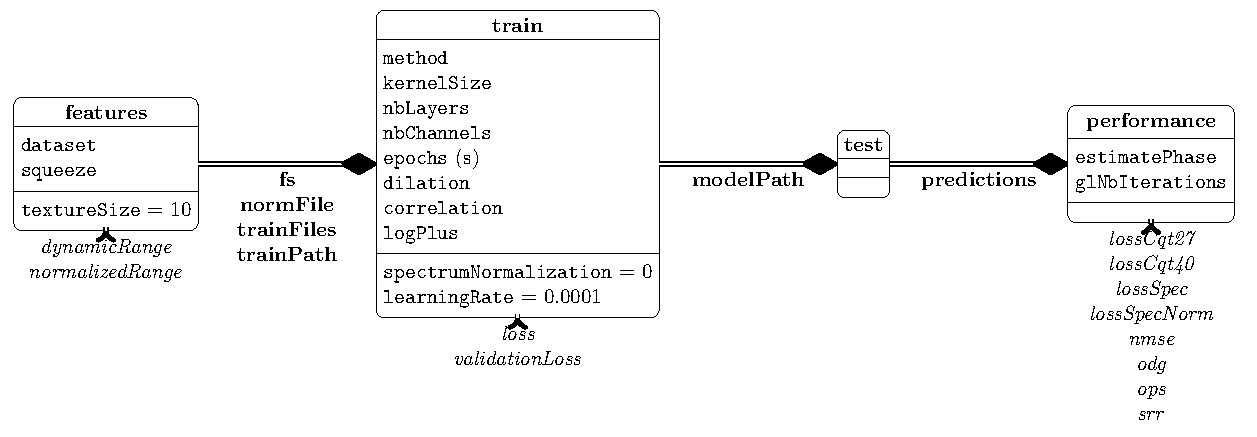
\includegraphics[width=\textwidth]{factors}
La commande \mcode{geometricShape('f')} génère un diagramme où les éléments principaux de l'expérimentation sont visibles (étapes de traitement, facteurs, données sauvegardées, observations).
\end{marginfigure}

Une fois l'implantation effectuée, le traitement est effectué avec la commande \mcode{'do'}. Par exemple, la commande
\begin{lstlisting}
geometricShape('do', 1);
\end{lstlisting}
demande le calcul de l'étape 1 pour toutes les conditions expérimentales (qui sont au nombre de 18). Il est souvent nécessaire de ne pas effectuer le plan expérimental complet (étude spécifique, reprise sur erreur, ...), le mécanisme de masquage est alors utilisé. Par exemple, la commande
\begin{lstlisting}
geometricShape('do', 0, 'mask', {[1 2] 0 1})}
\end{lstlisting}
demande le calcul successif des deux étapes pour les cylindres de rayon 2 et toutes les pyramides.

Après le traitement des deux étapes, le répertoire dédié au stockage des données de calcul et d'observations contient : \\
\begin{Verbatim}[fontsize=\scriptsize]
	base/color: blue, radius: 2, shape: cylinder_data.mat            space/color: blue, height: 2, shape: pyramid, width: 2_obs.mat
	base/color: blue, radius: 2, shape: cylinder_obs.mat             space/color: blue, height: 2, shape: pyramid, width: 3_obs.mat
	base/color: blue, radius: 4, shape: cylinder_data.mat            space/color: blue, height: 4, radius: 2, shape: cylinder_obs.mat
	base/color: blue, radius: 4, shape: cylinder_obs.mat             space/color: blue, height: 4, radius: 4, shape: cylinder_obs.mat
	base/color: blue, radius: 6, shape: cylinder_data.mat            space/color: blue, height: 4, radius: 6, shape: cylinder_obs.mat
	base/color: blue, radius: 6, shape: cylinder_obs.mat             space/color: blue, height: 4, shape: pyramid, width: 1_obs.mat
	base/color: blue, shape: cube, width: 1_data.mat                 space/color: blue, height: 4, shape: pyramid, width: 2_obs.mat
	base/color: blue, shape: cube, width: 1_obs.mat                  space/color: blue, height: 4, shape: pyramid, width: 3_obs.mat
	...							      ...
\end{Verbatim}

Ce n'est pas explicite dans cet exemple, mais les fichiers \mcode{\_data} dédiés au stockage des données de calculs sont souvent de taille plus conséquente que les observations qui elles ont vocation à rester de taille raisonnable pour pouvoir être transférées des machines de calcul aux machines de développement et de visualisation pour pouvoir être aisément analysées. Pour toute expérimentation de taille raisonnable, les noms de fichiers peuvent être compactés pour ne pas dépasser les 250 caractères requis par la plupart des systèmes de gestions de fichiers.

\`A la fin du traitement, les observations de la dernière étape de traitement sont affichées :
\begin{Verbatim}[fontsize=\scriptsize]
	Loaded data files dates are in the range: | 01-Apr-2019 10:15:55 || 01-Apr-2019 10:15:56 |
	    'shape'       'color'    'radius'    'width'    'height'    'baseArea'          'time'    'volume'
	    '---'         '---'      '---'       '---'      '---'       '---'               '---'     '---'
	    'cylinder'    'blue'     '2'         ''         '2'         '  12.55 (4.32)'    '0.22'    '   25.11 (8.63)'
	    'cylinder'    'blue'     '2'         ''         '4'         '  12.55 (4.32)'    '0.09'    '  50.22 (17.27)'
	    'cylinder'    'blue'     '2'         ''         '6'         '  12.55 (4.32)'    '0.00'    '  75.32 (25.90)'
	    'cylinder'    'blue'     '4'         ''         '2'         ' 50.85 (16.54)'    '0.00'    ' 101.70 (33.08)'
	    'cylinder'    'blue'     '4'         ''         '4'         ' 50.85 (16.54)'    '0.00'    ' 203.41 (66.15)'
	    'cylinder'    'blue'     '4'         ''         '6'         ' 50.85 (16.54)'    '0.00'    ' 305.11 (99.23)'
	    'cylinder'    'blue'     '6'         ''         '2'         '109.79 (33.75)'    '0.00'    ' 219.57 (67.50)'
	    'cylinder'    'blue'     '6'         ''         '4'         '109.79 (33.75)'    '0.01'    '439.14 (135.00)'
	    'cylinder'    'blue'     '6'         ''         '6'         '109.79 (33.75)'    '0.00'    '658.72 (202.50)'
	    'cylinder'    'red'      '2'         ''         '2'         '  11.92 (4.33)'    '0.00'    '   23.84 (8.66)'
	    'cylinder'    'red'      '2'         ''         '4'         '  11.92 (4.33)'    '0.00'    '  47.68 (17.32)'
\end{Verbatim}

L'accès à une grande diversité de mises en forme de l'exposition des observations utiles au discours est un élément nécessaire pour une expérimentation efficace. La plateforme \explanes dispose d'un grand nombre de fonctionalités conçues pour permettre une certaine flexibilité dans leurs usages.

Par exemple, ce dernier affichage peut être ré-obtenu grâce à la commande suivante :
\begin{lstlisting}
geometricShape('display', 2, 'expose', '>', 'mask', {[1 2] 0 1});
\end{lstlisting}
La commande :
\begin{lstlisting}
geometricShape('display', 2, 'mask', {1 0 1},...
 'expose', {'t', 'obs', 2});
\end{lstlisting}
affiche les volumes (observations 2) de l'étape 2 pour chaque cylindre de rayon 2 triés par la première observation sélectionnée. La fonte rouge indique la plus haute valeur, et les valeurs en gras, celles qui ne sont pas statistiquement différentes, au sens d'un t-test par paires effectué entre les observations de la condition expérimentale et celle correspondant à la plus haute valeur.

\begin{margintable}
\caption{Visualisation sous forme de table \LaTeX.}
\begin{tabular}{llc}
color & height & volume \\
\hline
blue & 2 &  26.12$\pm$9.30 \\
blue & 4 & 52.23$\pm$18.60 \\
blue & 6 & \textbf{\textcolor{red}{78.35$\pm$27.90}} \\
red & 2 &  24.61$\pm$7.54 \\
red & 4 & 49.23$\pm$15.07 \\
red & 6 & \textbf{73.84$\pm$22.61} \\
\end{tabular}
\end{margintable}

Dans notre exemple, même si le cylindre bleu est plus volumineux que le rouge, cette différence n'étant pas significative, on peut en conclure expérimentalement que la couleur n'influe pas sur le volume. Une fois la phase d'analyse des résultats effectuée, nous pouvons alors communiquer les résultats grâce à la production de rapports d'expérimentation. Quelques exemples de rapports d'expérimentation pour des expérimentations plus ambitieuses sont disponibles sur le site du projet \textsl{expLanes}.


Je me suis attaché à décrire ici une contribution personnelle à une problématique d'importance qui, sans prétendre viser à l'universalité, propose une systématisation de l'étape d'expérimentation de la méthode scientifique. Je présente dans la section suivante des éléments de réflexion concernant la fragile et dernière étape de la méthode scientifique et comment ce type de contribution peut amener à son amélioration dans le contexte scientifique actuel.

\section{\nmu La revue par les pairs} \label{sec:pairs}

Outil indispensable à la communauté scientifique, elle comporte néanmoins des risques pour le chercheur, c'est en effet à ce moment que les fruits de son travail sont exposés, à la critique, à l'utilisation abusive, ... C'est aussi une formidable opportunité pour voir son travail servir de base pour la recherche future.

On assiste actuellement à une \og crise \fg de la revue par les pairs ou plus exactement une crise de la publication d'articles, principalement à cause d'une normalisation d'une expression anglo saxonne "publish or perish" qui est, dans un nombre toujours plus grand de pays, devenue loi. Les nouveaux moyens numériques de diffusion facilitant cette inflation, le chercheur doit passer beaucoup de temps à écrire, mais aussi à relire, des articles dont le contenu s'allège en conséquence. En considérant que le nombre de personnes dédiant leur carrière à la recherche scientifique est resté stable durant ces 50 dernières années, les dernières estimations de l'évolution du nombre d'articles publiés sont préoccupantes\cite{bornmann2015growth}.

\begin{marginfigure}
  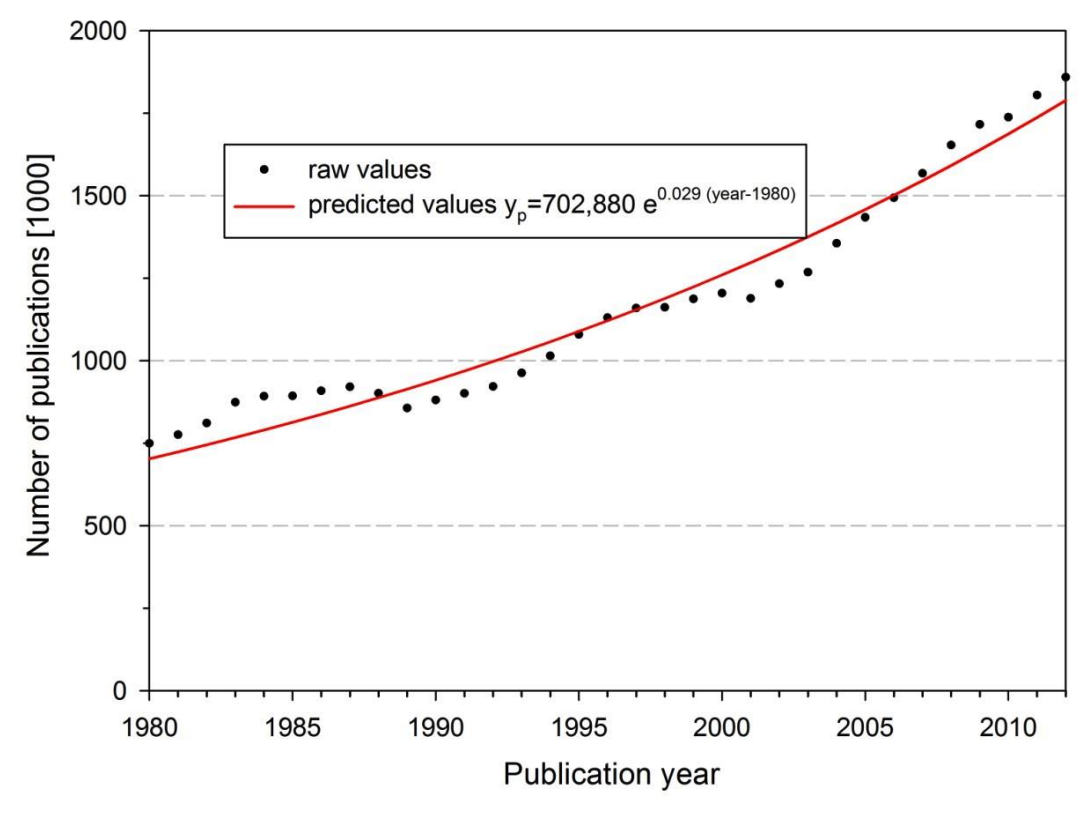
\includegraphics[width=\textwidth]{nbArticles}
  \caption{Estimation de la croissance du nombre de publications scientifiques.}
\end{marginfigure}

A ceci s'ajoute la position maintenant indéfendable des éditeurs qui, par abus de position historique, ne facilitent pas l'évolution nécessaire. Comment expliquer au contribuable les sommes demandées au chercheur pour l'archivage de ses articles (actuellement environ 1500 euros pour un fichier d'une dizaine de Mo). Il est malheureusement difficile pour un chercheur de prendre la décision de manière unilatérale de prendre des dispositions alternatives.

Comme tout moment de crise, de nouvelles opportunités émergent également qui pourraient amener à une nouvelle implémentation de cette dernière étape de la méthode scientifique qui soit plus respectueuse du chercheur et également plus effective pour la communauté. \marginnote{J'éviterai ici toutes questions concernant l'évaluation du chercheur, les produits de l'étape de la revue par les pairs n'étant pas à mon sens un outil approprié pour cet objectif.}

Dans une tradition issue de la physique expérimentale, la revue par les pairs se base sur la production d'une description aussi précise que possible du protocole expérimental et d'une discussion plus ou moins approfondie sur l'interprétation que font les auteurs sur les résultats obtenus. Ce format \og article \fg est motivé par le fait que l'environnement expérimental est très coûteux à mettre en place et difficilement transposable. Par accumulation d'expériences avec des protocoles expérimentaux d'une spécificité plus ou moins contrôlée, la communauté s'approche de ce que l'on peut être raisonnable de penser être la vérité. Un exemple particulièrement illustratif de ce processus est montré sur la Figure \ref{fig:copper} montrant une série de mesures de la conductivité du cuivre en fonction de sa température. Par l'accumulation et la réduction de mesures effectuées indépendamment, notre connaissance du phénomène observé s'affine.

\begin{marginfigure}
  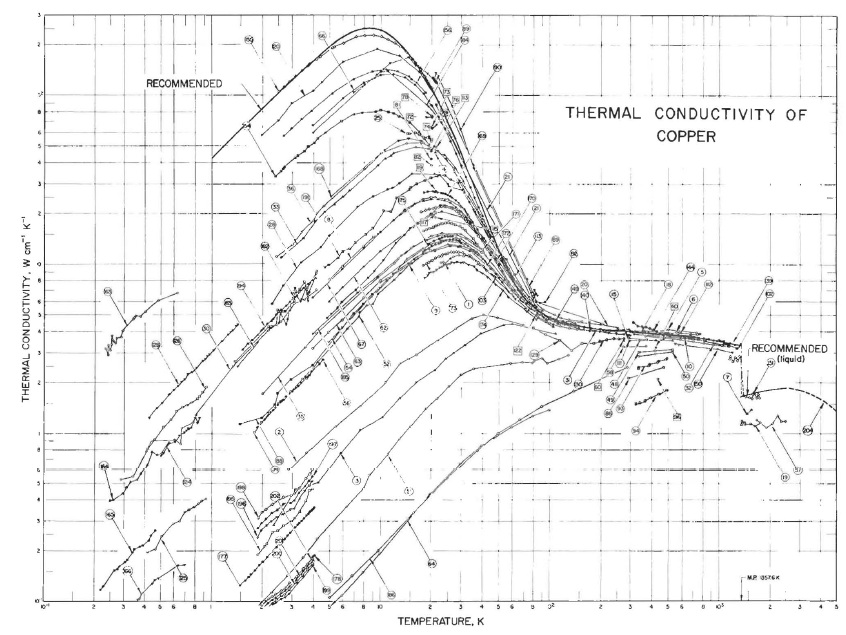
\includegraphics[width=\textwidth]{copper}
  \caption{Mesures de la conductivité du cuivre en fonction de sa température. Chaque ligne pointée par une bulle numérotée désigne les mesures publiées dans un article donné.}
  \label{fig:copper}
\end{marginfigure}

Dans le domaine de la sciences des données, on peut considérablement accélérer le processus de reproduction et d'extension, car il est plus aisé de mettre en place le paradigme de la recherche reproductible. En suivant la définition séminale de Donoho\marginnote{"An article about computational science in a scientific publication is not the scholarship itself, it is merely an advertising of the scholarship. The actual scholarship is the complete software development environment and the complete set of instructions which generated the figures." \\—D. Donoho} et en l'étendant au cadre des sciences des données, on peut considérer qu'une contribution scientifique doit pour cela être composée:
\begin{enumerate}
  \item des données servant de base à l'expérimentation;
  \item de l'implémentation qui, en fonction de ces données, produit les éléments quantitatifs discutés dans le compte rendu;
  \item d'un compte rendu d'expérience ou article détaillant les hypothèses, le protocole expérimental et les conclusions.
\end{enumerate}

Concernant la pérennité des données et de l'article, ces données numériques dites \og statiques \fg ne posent pas de challenge particulier. Ce n'est malheureusement pas le cas du code informatique car il dépend d'une pérennité de l'interprétation de ce code sur les machines contemporaines.L'archivage et la maintenance du matériel qui a servi aux expérimentations n'est pas dans le cas général envisageable. Les difficultés de réplication pour cause d'obsolescence matérielle et logicielle sont endémiques de la recherche en sciences des données car cette activité se situe généralement dans des secteurs de pointe évoluant très rapidement\marginnote{Je citerai pour exemple l'évolution actuelle des bibliothèques de calcul sur unité de calcul graphique comme la bibliothèque \textsf{cuda}\textsuperscript{\tiny\textregistered} développée par \textsf{nvidia}\textsuperscript{\tiny\textregistered}. Indispensable pour tout traitement efficace d'architectures profondes, cette bibliothèque est propriétaire et les versions antérieures ne sont plus maintenues après seulement quelques années.}.

Il reste que, bien souvent, une maintenance régulière du code par les auteurs au cours du temps permet de préserver un certain niveau d'équivalence des résultats. Il est alors pour cela très utile de disposer d'un code qui soit bien structuré et facile à maintenir. Cette maintenance sera également grandement facilitée par le choix judicieux des dépendances du code informatique publié. Si la phase d'expérimentation nous incite généralement à essayer de nombreuses approches, dont certaines très novatrices mais potentiellement instables et faiblement maintenues, il convient au moment de la publication de réfléchir à un bon équilibre entre apport technique et pérennité.

Garantir une reproducibilité complète pour un temps long de toutes ses productions est un défi probablement trop coûteux pour le chercheur. Il convient néanmoins de réfléchir en amont à cette problématique et d'allouer l'énergie nécessaire aux projets qui trouvent intérêt dans la communauté\marginnote{Les plateformes de développement collaboratif comme gitHub sont à ce titre particulièrement adaptées car elles permettent d'être informé de l'intérêt que porte la communauté aux travaux publiés et d'assister les collègues lors des tentatives de réplication.}.

Même si l'implémentation particulière n'a pas vocation à être pérenne, il est bien évident que si les auteurs ont suivi un protocole expérimental canonique avec un effort de clarté et de concision dans l'implémentation, la réplication sera bien plus accessible. L'utilisation de cadres computationnels comme \explanes pour mettre en place ce protocole expérimental est d'intérêt car ils permettent d'encourager de bonnes pratiques en facilitant leurs mises en place.

Techniquement parlant, il est par contre aisé que les données expérimentales soient stockées de manière pérenne sur des plateformes publiques\footnote{Les plateformes de type \textsf
{archive} (\url{https://archive.org}) ou \textsf
{zenodo} (\url{https://zenodo.org}) sont de bons candidats.}. La contrainte ici n'est pas d'ordre technique mais légale. L'usage de données publiques doit donc être encouragé par la communauté.
